\documentclass[../../lecture_notes.tex]{subfiles}

\begin{document}

\noindent A few things set two-player games apart from standard search problems:
\begin{itemize} [itemsep=0mm]
	\item Opponents — the next stage is unpredictable, so we need a strategy
	\item Time Limits — search time is limited, so a good, fast result is better than a perfect slow one
\end{itemize}

\subsection*{Formulating 2-Player Games As Search}
\noindent Consider Chess; we have two major issues to address:\\
\indent The effective branching factor is roughly 35, so the tree is huge.\\
\indent We don’t know the moves the opponent will make.\\

\noindent What we need is a \textbf{\underline{conditional plan}} (equivalent to a strategy).\\
This solution will thus include:
\begin{enumerate} [itemsep=0mm]
	\item a goal state at every leaf
	\item an action at each of our turns
	\item a path for each of the foe’s choice
\end{enumerate}

\subsection*{Minimax}
\begin{centering}
\noindent \begin{figure}[H] 
	\captionsetup{labelformat=empty}
	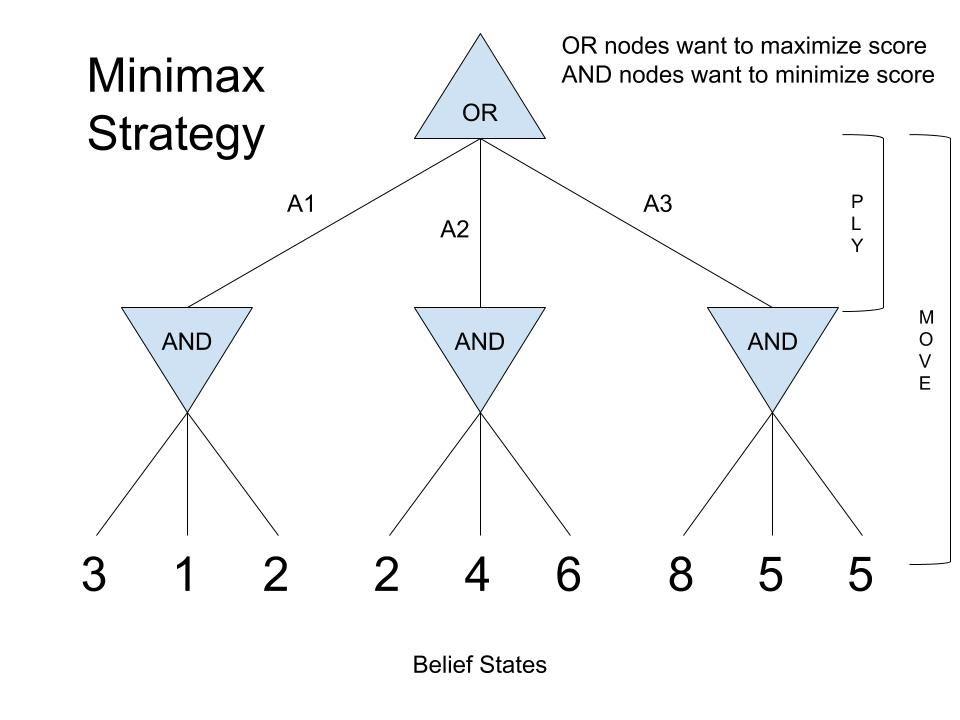
\includegraphics[width=0.8\textwidth] {minimax} \caption{}
\end{figure}\end{centering}

\noindent We only need an algorithm which chooses from \{A1, A2, A3\}, since we can reapply each turn.\\
We assume that the opponent is perfect, since if they aren’t we will only do better.\\
If choose $A_1$ — then our opponent will choose 3, thus we want to choose the best worst case.\\
\\
We consider this approach bottom-up, since we compute scores starting at the bottom.\\
How do we build the tree?  DFS.\\
Recall space = O(bm) \& time = O($b^m$)\\
\\
Consider chess: it has a branching factor of roughly 35.\\
The time limit is often 100 seconds.\\
We can generate $10^4$ nodes/second.\\
$\implies$ choices = $log_35(10^6) = 4$, so our approach is 2 PLY.
Is that good?\\
\indent 4-ply look ahead — human novice\\
\indent 8-ply look ahead — human master\\
\indent 12-ply look ahead — Kasparov, Deep Blue\\
Thus our method is not nearly sufficient.\\
\\
We need to “cut m” via an \textbf{\underline{evaluation function}}\\
\indent $\equiv$ a function which attempts to approximate the minimal node value.\\
Requirements for the function:
\begin{enumerate} [itemsep=0mm]
	\item agrees with the utility function on terminal nodes
	\item is efficient to compute
	\item is accurate in premise
\end{enumerate}
\noindent Note that this may lead us to cut off paths at different steps.

{
\floatsetup{capposition=beside,capbesideposition={right}}
\begin{figure} [H]
	\captionsetup{labelformat=empty}
	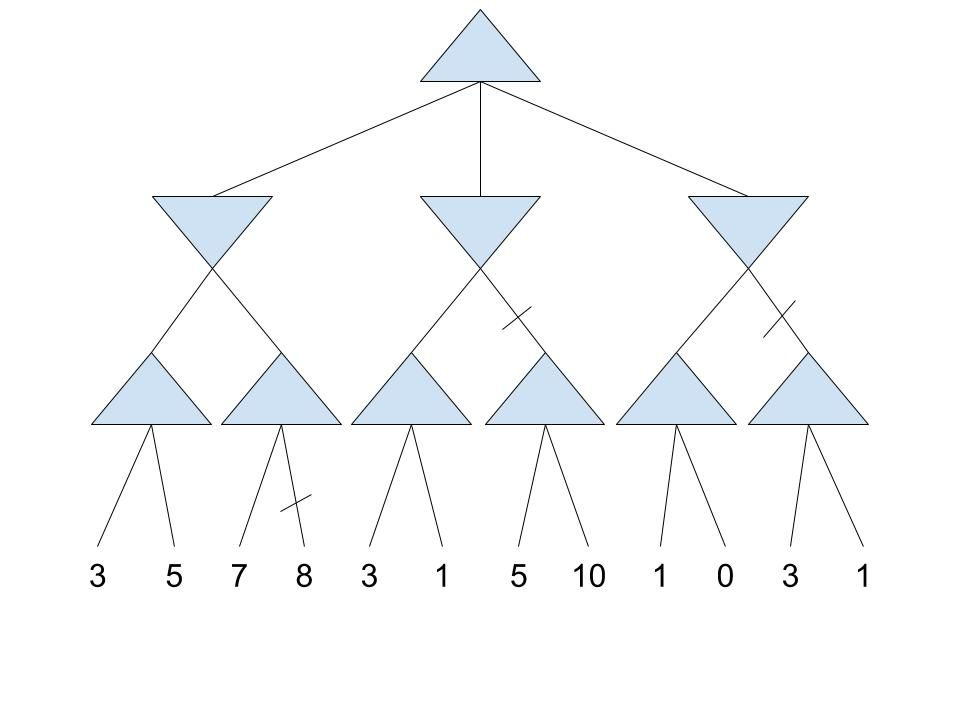
\includegraphics[width=0.5 \textwidth] {abpruning}
	\caption{We can skip any value lower than the min!\\
			This is called \textbf{\underline{alpha-beta pruning}} \\
			\indent (alpha for max, beta for minimum).\\
			\noindent Our behavior is dependent on the type of node:\\
			\indent min node — examine children lowest-first\\
			\indent max node — examine children largest-first\\
			\noindent The gain depends on value order.\\
			$\implies$ with a-b pruning, $T = O(b^{m/2})$.\\
			This is up to twice as deep!\\
			This is the best case, the average is $O(b^{3m/4})$.\\
			\newline \newline \newline
	}
\end{figure} 
}

\subsubsection*{Stochastic Search}
\noindent This strategy cannot work for games of chance since we cannot predict our choices.\\
We can instead use probabilities to weight the values.\\

{
\floatsetup{capposition=beside,capbesideposition={right}}
\begin{figure} [H]		
	\captionsetup{labelformat=empty}
	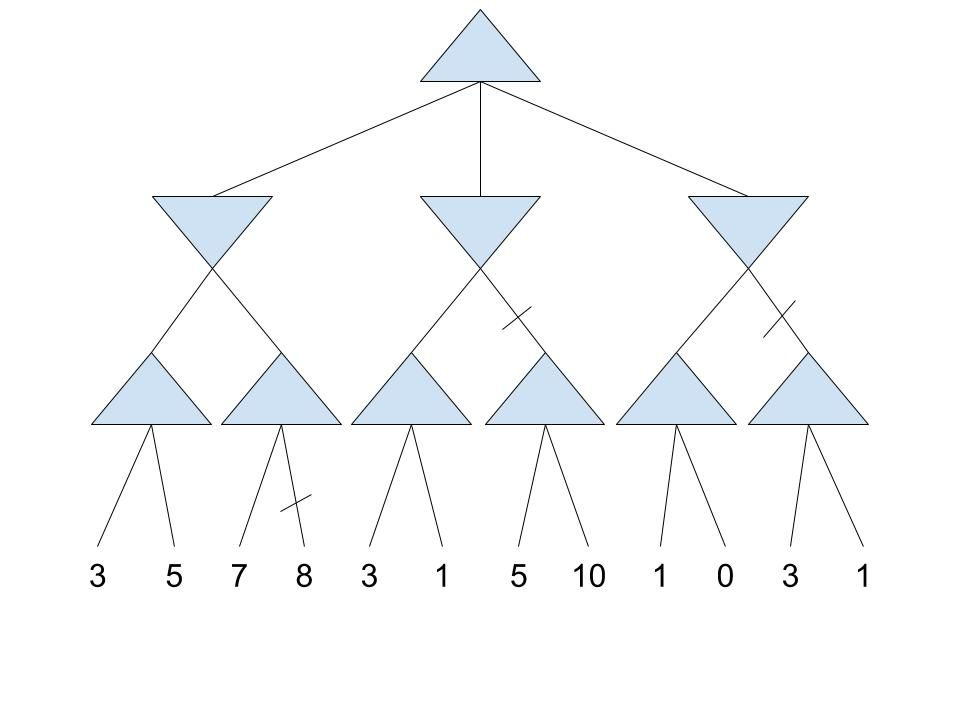
\includegraphics[width=0.5 \textwidth] {abpruning}
	\caption{\noindent Our choice of cutoff is very important:\\
		\indent A depth cutoff in a search (here 2) must be \textbf{\underline{quiescent}}\\
        		$\equiv$ unlikely to drastically change values.\\
		\indent A bad cutoff may fall victim to the \textbf{\underline{horizon effect}}\\
	        $\equiv$ when negatives are pushed just past the cutoff.\\
		\indent We address this by logging clearly great moves.\\
		Time complexity: $O(b^m n^m)$ for n distinct events.\\
			\newline \newline \newline
	}
\end{figure} 
}\medskip

\subsection*{Additional Game Strategies}
\noindent At the beginning or the end of a game, it may be more practical to do a table lookup.\\
\indent $\equiv$ create a policy (a mapping from every single state to its optimal reachable state).\\
\indent We can then do a \textbf{\underline{retrograde}} 
	($\equiv$ bottom up) search from an ideal to choose our action.\\

\subsubsection*{Probabilistic \& Perfect Information}
\begin{enumerate} [itemsep=0mm]
	\item define a chance node which holds the expected value of its children
	\item \textbf{\underline{Monte Carlo Simulation}} $\equiv$ estimate values by win percentage
\end{enumerate}

\subsubsection*{Probabilistic \& Imperfect Information}
\begin{enumerate} [itemsep=0mm]
	\item \textbf{\underline{averaging over clairvoyance}} $\equiv$ solving over all possible “rolls”\\
	            This has the negative tendency to avoid moves that gain the player information
	\item introduce randomness for an equilibrium solution
\end{enumerate}

\end{document}